
\vspace*{10mm}

The following appendices contain information about the old scheduler of pyProCT, the analysis tools used, the work methodology and temporal planning, an estimated budget an sustainability issues and, finally, the list of all manuals and documentation used.

First chapter relies on a simple tic-tac-toe game to explain the scheduler and use analysis tools. This approach helped to understand how to use them in a more limited context where it's easier to catch bugs or possible problems prior to their use on pyProCT. The program is first described on the following chapter to put the reader in context. Afterwards that small program is refactored with pyScheduler. Next section uses the modified code to tests extrae and paraver analysis tools on its different versions (sequential, MPI and python's multiprocessing).

Appendix \ref{app:problems}. describes all the problems that are not directly related to the pyCOMPSs refactor. It is composed of issues arisen by python versions, encodings and configurations.

Next two appendices are related to how the project was planned and developed. In them the reader will find the work methodology used (Appendix \ref{sec:methodology}) and the temporal planning (Appendix \ref{sec:temporal_planning}). 

On Appendix \ref{sec:budget} the estimated cost of the project is given. It is divided into human, hardware and software resources. Next chapter, (appendix \ref{sec:sustainability}) gives an opinion about the social, economic and environmental impact of the work done.

Last appendix, \ref{sec:docs}, chapter contains all the documentation used. Here the reader will find the tools' manuals, readmes, tutorials and all the information sources which do not belong to the bibliography.

\chapter{Scheduler and Performance Tools}
\label{chap:ttt}

\section{Motivation}

This section explores pyProCT's scheduler and the tools necessary to analyse its performance. An small sequential testing program was written in order to test it all on a much smaller scale. The next sections' decriptions rely on it to explain the scheduler and tools. More precisely, first section will describe the program to put the reader in context. On the second section I will parallelize the program with the scheduler. Last two sections will describe the analysis process: first the instrumentation for generating traces and then the visualization tool. During the process I will try to find possible problems that may arise due to the parallelization, like the reproducibility on random algorithms or results' validation, which could complicate the posterior work on pyProCT.


\section{Test program description} 
The developed program was an command-line implementation of the popular game Tic-tac-toe. It suited quite well the project needs because it featured good parallelization options, stochastic elements, a clear turn structure (easing up the first analysis trials), variable-size parametrized tasks and automatized execution (having two AI playing).

\hyperref[fig:tic-tac-toe]{Figure \ref{fig:tic-tac-toe}} shows a simplified version of the program's execution flow. All the logic handling which player's turn is, how the board is marked and some other parts have been omitted because they are not relevant. 

For each turn, while the game is not finished, the program calls the \textit{Player} class' \textit{play()} function. The algorithm implementing the AI moves is a montecarlo-like method. It randomly simulates a big number of games for each available cell and then choses the cell with the best score.

To do this it first gets all the free cells, then for each available one it calls the exploration\_handler method. This method in turn calls mark\_an\_explore a number of times (this number is defined by the ITERATIONS parameter which is a command-line argument) with a copy of the game board. Basically, mark\_and\_explore first the cell passed as parameter and then fills randomly the copied board, till the game is finished (either by a player winning or a draw), returning the cell and the id of the winning player or a 0 if there is a draw. The list of winnig id's is then returned to the montecarlo function. Afterwards we initialize the score value for each available cell with infinity. Then for each tuple containing a cell and the winner of that simulation we increment the score of the cell if the player has won or decrease it if the player has lost (the algorithm could modify the score for draw results). The actual increment/decrement values can be tuned but it's not relevant for testing purposes. 

\section{PyScheduler}

Once the sequential program was ready, next step was to decide how to refactor it with pyScheduler (pyProCT's scheduler). The decision was to consider each \textit{exploration\_handler()} function as a task to see how their size affects the performance of the scheduler. The ITERATIONS parameter allows to change the number of iterations performed inside \textit{exploration\_handler()} so this was deemed the best option. 

The selected scheduler has three scheduling types, one sequential and two parallel: 

\begin{description}
\item [Serial,] which executes the task sequentially.
\item [ProcessParallelScheduler,] which uses python's multiprocessing module.
\item [MPIParallelScheduler,] which uses mpi4py for the parallelization.
\end{description}

The usage of the scheduler is simple. For each task we have to call the \textit{add\_task} method providing the following information:

\begin{description}
\item [Task name:] a unique task name.
\item [Dependencies:] a list of this task dependencies (which must be a list of other tasks names).
\item [Description:] a description of the task.
\item [Target function:] the name of the function to be executed.
\item [Function kwargs:] the list of the keyword arguments which need to be passed to the target function.
\end{description}

Once the task list is completed we just need to call the \textit{run()} method of the scheduler. The method will return a list with the execution results of each task.

For the tic-tac-toe these are the values for the queued tasks:

\begin{description}
\item [Task name:] ExplorationXY (being X, Y the coordinates of the cell to be explored).
\item [Dependencies:] [ ] (the empty list because there are no dependencies among different explorations).
\item [Description:] Montecarlo exploration.
\item [Target function:] self.exploration\_handler (as we are inside Player class namespace we must add the self).
\item [Function kwargs:] {"x": x, "y": y, "board": board} (being X, Y the coordinates of the cell to be explored, and board the current state of the game).
\end{description}



\section{Instrumenting with Extrae}

\label{sec:instrumentation}

Next step was to start using the analysis tools. The decision was to use the  \textbf{Extrae + Paraver} combination. Extrae \footnote{ Find extrae documentation on the performance tools section of \ref{sec:docs} .Documenation} is the package used for instrumenting the code; Paraver \footnote{ Find paraver documentation on the performance tools section of \ref{sec:docs} .Documenation} is the tool used to visualize the traces generated by Extrae. These tools have been both developed at the BSC to be used together. We chose them because of the Extrae support to python, the offered assistance and proximity of the tools' experts and the fact that they are both installed and configured on MareNostrum III, which is our target execution platform.

Extrae offers two different ways to instrument the code: automatically instrument functions (providing a list of functions to the extrae XML configuration file) or including the extrae module (import pyextrae)  and emit specific events inside the code with \textit{pyextrae.eventandcounters(type, value)}. 

The basic usage of the first, which  does not require any changes on the code, instruments the entry and exit points of the functions. More complex behaviours are also available but for these tests the basic one is enough. 

The second one just needs to add the mentioned function call wherever we are interested to emit an event.

To start, \textit{play, montecarlo} and \textit{exploration\_handler} methods were set to be automatically instrumented and two more events were manually added: one before the scheduler intialization and task addition and one just after the scheduler \textit{run()}. On the sequential version \footnote+{ From now, "sequential" will refer to the schedulerless version, "serial" to the one with the sequential scheduler, "parallel" for the one using ProcessParallel and "mpi" for the mpi4py one} this corresponds to before and after looping through the available cells (calling \textit{exploration\_handler} on each iteration).

Support for python is only available from version 3.0 onwards and it's not fully tested so we faced some problems. For the sequential and serial versions everything went well, the traces  were correct and they could be visualized with Paraver. For the parallel version we were not able to extract correct traces as extrae was not able to detect the parallelization method. When I tried the MPI version it didn't work either for two reasons. On one hand, adding the user functions' automatic instrumentation made the whole execution to end with a segmentation fault without generation the traces. On the other hand, using just the event emit method, the visualization showed just one thread. 

After meeting with BSC people we managed to solve the issue. The problem was that extrae used a sequential-tracing library, so it could not detect the mpi multiple threads. To solve it we substituted this sequential library with an mpi-tracing one. After some work on their part the first issue was also solved by changing some values on \textit{Extrae\_define\_event\_type}. 

For the parallel implementation with multiprocessing this approach wasn't supported. They gave me some ideas to try but to no avail. I linked extrae with a number of different libraries, such as the pthreads one, to see it they were able to hook themselves to the python multiprocessing threads but it didn't work. I left the issue open and went forward. Fortunately, after working on the new tracing system for pyCOMPSs at the BSC, I managed to develop a workaround tracing system albeit quite more rudimentary and inconvenient to use. Extrae has a command line usage of which I used two basic commands:

\textit{extrae-cmd init node slots}

\textit{extrae-cmd emit slot event\_value event\_type}, 

A python class wrapper was created for this two commands. This way it's possible to reuse it to instrument pyProCT later. This class deals with the extrae paths and concurrency as well as providing a easier interface to call from python. To use it first it is necessary to initialize each used node with an ID and the number of processes/threads it will contain. Then for each event we want to emit we specify it's ID (which must be positive and smaller than the number of threads we set for that node) and the value and type of the event. 

The first trials raised a segmentation fault; knowing that emitting an event with an out-of-range thread ID raises a segmentation fault hinted that the initialization was not correct. Because this extrae usage is not the recomended nor normal approach there is no documentation for it nor examples for it. After several attempts we met with the extrae team. Working with them we found out that the segmentation fault was caused by a bug on the used version. Kindly they fixed it and made a custom package for this project's use. With it, basic instrumentation for the parallel (with python-multiprocessing) version was finally achieved. This is limited to emit events and can not produce the advanced visualizations and results achieved on the serial and MPI version.

\begin{landscape}
\begin{figure}
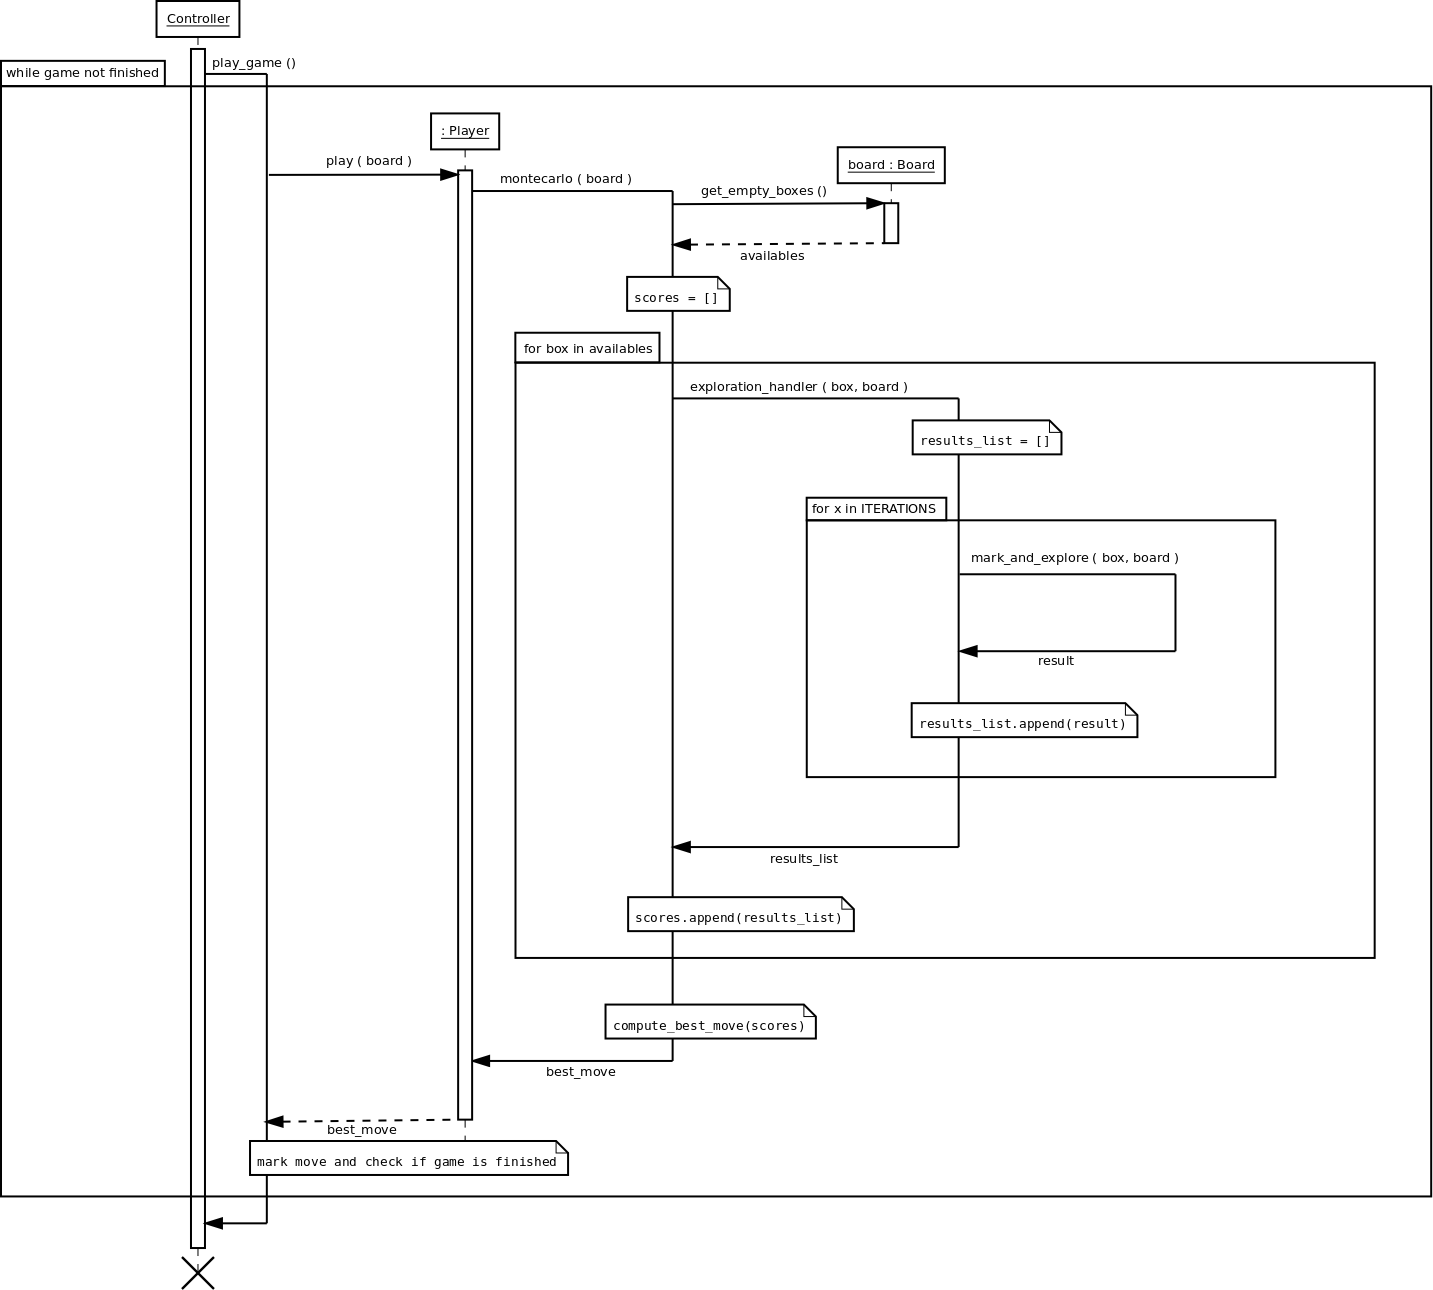
\includegraphics[width=20cm]{img/tic-tac-toe.png}
\caption{Tic-tac-toe Execution Flow}
\label{fig:tic-tac-toe}
\end{figure}
\end{landscape}


\section{Visualizing with Paraver}


Once generated the trace file the next step is to analyse them with the visualization tool Paraver.

First thing was to create a configuration file that would show the instrumented user functions (montecarlo, play and exploration\_handler on this program). To do so one needs to configure the event filter to show only events of the type 60000100 (which is the type assigned to instrumentated user functions), and the semantic options to show the last event value (that is the values identifying the functions) in a stacked composition. Thanks to the ability of copy/paste time info from a graphic we can quickly compare different traces.

 \hyperref[fig:fig:ttt-python-funcs-seq]{Figure \ref{fig:ttt-python-funcs-seq}} shows the visualization of three executions of the tic-tac-toe, all of them with 500 iterations. The first is an schedulerless version, the second with the serial scheduler and the last one with an MPI scheduler. At the time of writing the parallel/multithreading scheduler can't be instrumented, as this is a demo section of the Paraver capabilities we have considered that leaving the parallel version out will not harm the purpose of this section. Dark blue corresponds with exploration\_handler function, white with montecarlo, red with play and light blue the time outside these three functions. The MPI version has more labels but for the current section the details aren't important. We can see on the figure that the serial scheduler has an important overhead, making it slower than the schedulerless version, but the MPI scheduler is quite faster.
 
 
\begin{figure}[h]
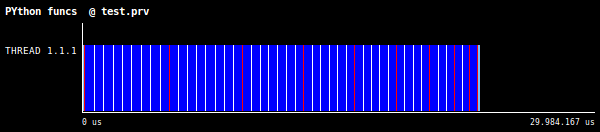
\includegraphics[width=\textwidth]{img/ttt_500_python_funcsG11.png}
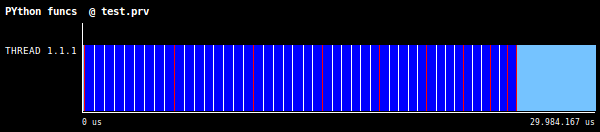
\includegraphics[width=\textwidth]{img/ttt_500_python_funcsG12.png}
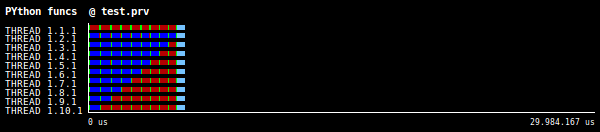
\includegraphics[width=\textwidth]{img/ttt_500_python_funcsG13.png}
\caption{Tic-tac-toe 500 iterations executions}
\label{fig:ttt-python-funcs-seq}
\end{figure}


Paraver has a wide range of configurations to visualize MPI information (see \hyperref[fig:fig:ttt-mpi-IPC]{Figure \ref{fig:ttt-mpi}} ), useful execution time or IPC. We can inspect data in timeline or tabular form but also with the aid of other tools such as the Clustering. With this tool we can cluster the results to obtain, for example, a graphic relating the executed instructions and the IPC. Thanks to this we can bypass analysis problems related with the time where, sometimes, an increase or unbalance in the workload depends on the IPC rather than the number of instructions. On \hyperref[fig:fig:ttt-mpi-IPC]{Figure \ref{fig:ttt-mpi-IPC}} we can see that the most computation-intensive areas associated with the exploration\_handler function (in blue on  \hyperref[fig:ttt-python-funcs-seq]{Figure \ref{fig:ttt-python-funcs-seq}}) have a good efficiency. 
 
 
\begin{figure}[h]
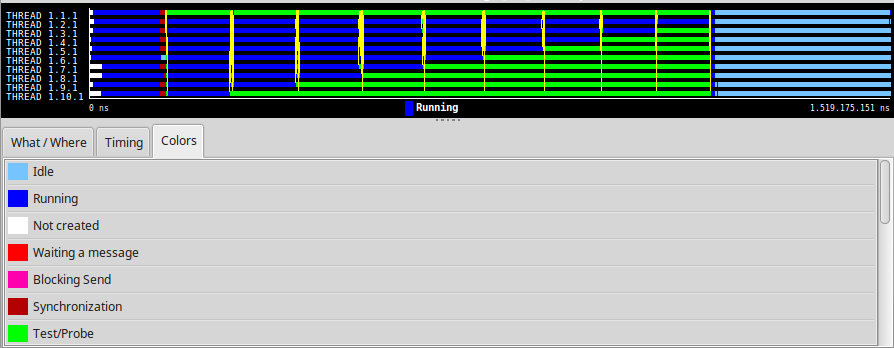
\includegraphics[width=\textwidth]{img/New_window_1_2DZoom_range_[1,6]@test.png}
\caption{Tic-tac-toe MPI information for a 500 iteration execution}
\label{fig:ttt-mpi}
\end{figure}


 
\begin{figure}[h]
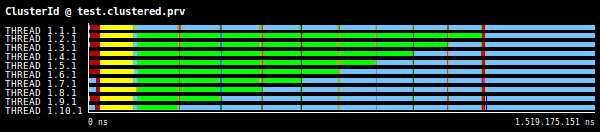
\includegraphics[width=\textwidth]{img/cluster_graph_mpi.png}
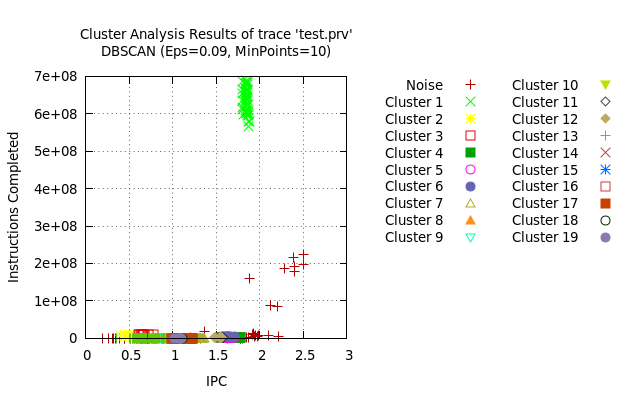
\includegraphics[width=\textwidth]{img/cluster_mpi_IPC.png}
\caption{Tic-tac-toe timeline and clustering for 500 iteration MPI execution}
\label{fig:ttt-mpi-IPC}
\end{figure}


\chapter{Problems}
\label{app:problems}
\section{Python versions}

This first issue arose when trying to compile and link the development version of pyProCT. It is related with MN3's modules environment. By default, on login, MN3 has 2.6.9 python, however this version is not available to be loaded through the modules; it's only available when no other python has been loaded by the .bashrc file nor manually with \textit{module load PYTHON}. 

pyProCT depends on python 2.7.3 which can be loaded with the modules. At first I compiled and installed it with the default release (2.6.9) with setup.py. On MN3 I had to add a custom installation path (with \textit{--prefix=PATH} option) to setup.py because I have no permissions to write into the default installation directory. After installing it I found out that pyProCT can not be run under python 2.6.9 so I started again all the installation process with 2.7.3 once I figured what was causing the error. 

The new installation arose the next issue

\section{Unicode encoding}

The message error of this bug was:

\textit{undefined symbol: PyUnicodeUCS4\_DecodeUTF8}

This is caused when trying to use software build with UCS4 on a UCS2 python version. On MN3 each installation uses a different one.

\begin{itemize}
\itemsep0em 
\item Python 2.7.3 $\rightarrow$ UCS2
\item Python 2.6.9 $\rightarrow$ UCS4
\end{itemize}

Python is not a compiled language, so this compilation problem actually comes from the Cython modules integrated into pyProCT. This meant that the new installation (which used the same folder as source) was not recompiling the Cython modules even after issuing a clean command so I cloned the repo again and started from scratch. This time everything ran smoothly. As a curiosity if pyProCT is build with python2.6.9 it can be used with python2.7.3 (although rising some compatibility warnings).

\section{Prody and extrae}

When trying to generate traces with extrae (for MPI and sequential version) I got a Prody error. When trying to resize any kind of structure Prody detects that there is more than one reference to that structure (introduced by the instrumentation) and fails to do the resize. To avoid this I had to manually modify the Prody package and, for each resize, add the parameter \textit{refcheck=False}. This error is raised in order to avoid integrity problems when an object has more than one reference; however we know that the instrumentation will not modify nor actively use those structures so we can safely disable the reference's check. 

\section{Size of floats}

This issue was raised by some datasets. Depending on the computer and data when I try to recreate the condensed matrix on the pyCOMPSs task I get an incompatible format error. This happens when numpy stores the matrix data (in list format) as floats with 32 bits. The matrix constructor however requires that data to be in floats with 64 bits. To overcome this I found that numpy arrays have a method, \textit{data\_view('float64')}, to select which type of elements should be returned and thus allowing me to always format them as 64-bit floats and solve the issue.

\chapter{Work Methodology}
\label{sec:methodology}
There are many ways to try to optimize pyProCT, some of them complex enough to be a full project. Due to the limited time and the loop structure of the development, we decided to use an Scrum based methodology. We set time-variable cycles at the end of which the work was evaluated. 

Paraver and Extrae have been used for traces' analysis; pyProCT-regression, to validate the new implementation. These tools, as well as pyCOMPSs and pyProCT, are still on development and not fully tested. This scenario suited best an Scrum methodology. Having cycles meant that it was easier to evaluate if some trials led to a dead-end, were best implemented on another way or, simply, were not feasible because they were unsupported.

Each cycle was bound to an specific modification. To begin each cycle we analysed first the state of the project and how previous work affected the code to define the next goal and the expected results. Once decided the work plan, we proceeded to it's implementation. 

Once finished we checked if the goals were achieved. The duration of each cycle was variable because the complexity of each optimization can vary a lot. This helped to keep track of the work and decide if a particular modification was taking too long or could not be implemented. It also reflected the possibility that an optimization did not improve the overall performance, case in which the results were analysed and reported nonetheless prior to planning the next work to be done.

This methodology takes into account how each modification affects the next one allowing a better planning. We deemed this approach better than  performing a full initial analysis and deciding at once all the optimizations to be implemented. 

To work on this project, a laptop with the text editor Sublime Text 3 was used. The computer had installed all the required software to run the code on the Mare Nostrum machine (through ssh), fork and manage the code versions with git, run the tests and instrument the code (for further details see both \ref{sec:hardware_resources} Hardware Resources and \ref{sec:software_resources} Software Resources sections).

\section{Limitations and Risks}


The reproducibility problem, defined as the impossibility to repeat an exact execution of the algorithm because of some stochastic parts, such as random initial parameters estimation for example, could difficult the validation and testing part. This could lead to a number of problems. First, the inability to use the black-box validation if two executions with the same data set lead to different results. This clearly affects all the parts of the process involving some kind of randomness. To control this, in case it  affects the testing process, I will try to eliminate the stochastic issues with random seeds and manual and fixed parameter estimation.

Another issue could be the time. To mitigate this problem the initial set-up phase before the SCRUM iterations has been added (see subsection \ref{subsec:setup} on Tasks Description). The goal of this is to automate the analysis, execution and all the other time-consuming tasks not related to the actual development of the optimizations. 

More problems such as the inability to correctly enqueue jobs to Mare Nostrum III will be addressed by counting on the BSC team and the project director. The usage of extrae and paraver tools could also be difficult. To overcome it, on the one hand, I went to a seminar about that tools. On the other hand I contacted the tools team to get their help when needed. This support is taken into account as an exterior consultant. 

At the present time COMPSs team is working on a brand new release (1.3). It has important changes with respect to the last one (1.2). The goal of this project to use, test and evaluate COMPSs so 

I decided that using the development version (1.3) would be more useful for the team and its performance is better than the old one. However, this new one is neither finished nor fully documented and tested. This is probably the major source of problems for this project.

Finally, the decision to work with the development version is the biggest risk of all because I can not finish my work if the release is not stable enough to run pyProCT. 

\chapter{Temporal Planning}
\label{sec:temporal_planning}


\section{Task List}

This section lists all the tasks to be performed.

\begin{enumerate}
\item Project Management
\begin{enumerate}
\item Project's Scope - 9h
\item Temporal Planning - 6h
\item Budget and sustainability - 3h
\item First Presentation - 6h
\item Context and Bibliography - 15h
\item Degree's specialization specification - 10h
\item Final document and presentation - 20h
\end{enumerate}
\item Software design description - 40h
\item Analysis tools' research - 40h
\item Common set up for all SCRUM cycles - 40h
\item SCRUM iterations - 960h control cycles
\begin{enumerate}
\item Initial analysis and optimization decision
\item Optimization development
\item Implementation measurements
\end{enumerate}
\item Global performance analysis - 40h

\item Project Writing and Defence Preparation - 80h
\end{enumerate}

\section{Tasks Description}


\subsection{Project Management}

This task is the responsible for the whole project planning and specification and covers all the deliverables of the GEP course.

\subsubsection{Resources list}

\begin{description}
\item [TexStudio,] \hfill \\ desktop application used for report writing
\item [GanttProject,] \hfill \\ desktop application for Gantt chart creation
\item [UPC Atenea,] \hfill \\ online platform for deliverables submission
\end{description}

\subsection{Software design description}

The project aims to optimize an already existing project. This means that the first thing to do before starting to work is to explore, execute and, in general, familiarize myself with the original code. This will lead to the design description of pyProCT software.

\subsubsection{Resources list}
\label{subsec:familiarresources}

\begin{description}
\item [Git and Github,] \hfill \\ to use the code we need a Github account to fork the original project repository. Once forked we need a git-able OS, in this case Linux Mint 17, to clone it.
\item [MareNostrum III account,] \hfill \\ for executing the code on the supercomputer and correctly assess it's performance as well as execution limitations for instrumentation purposes.
\item [SSH-able OS] \hfill \\ to establish secure shell connections to the MareNostrum III computer for the program execution.
\item [Paraver and other analysis tools,] \hfill \\ to ease the understanding process with execution diagrams. Also, on this first stage, I will start looking for the best available tools for the posterior analysis stage.

\end{description}

\subsection{Analysis tools' research}

Once the whole program execution and mechanics, the next step is to decide which analysis tools are going to be used. Paraver is going to be amongst them. This task needs to be done after getting familiar with the code because otherwise we could end up trying to use tools which are not compatible with the python version and packages used and the remote execution pipeline.

It is important to note that this is mainly a research stage. This means that no consistent code modifications are going to be performed, just the necessary ones to ensure that the tools work well with the code.

As a big part of the project is going to be analysis, we set up first this research stage and an implementation/instrumentation one in order to correctly address the importance of this matter.

\subsubsection{Resources list}
See \hypertarget{subsec:familiarresources}{Code Familiarization resources list~\ref{subsec:familiarresources}}.

\subsection{Common set up for all SCRUM cycles}
\label{subsec:setup}

Once I am familiar with the code and the analysis tools have been chosen, the next step will be to instrument the code for it's preliminary analysis. The instrumentation should be deep enough to test all the possible implementations to be done, regardless they are performed on the matrix distances calculation, task level or scheduler level.

On this stage we will also do a preliminar work aimed to automate and speed up as much as possible the code analysis and execution. On one hand, this will speed up the SCRUM iterations by automating the analysis and execution with tools like bash scripts, allowing us to focus on the actual development and analysis and avoid wasting time on repetitive task as graphs' generation or the remote execution. On the other hand, it will also help to avoid human errors on the execution parameters, analysis settings and environment configuration.

\subsubsection{Resources list}

The resources required for this stage are linked to the analysis tools decisions so they can not be listed until the first stage is finished.

However common resources for automation are required (i.e. bash scripts). The Linux Mint environment used provides this basic functionalities.

\subsection{SCRUM iterations}

As explained on the Scope of the Project document, the work flow will follow the analysis-implementation-analysis structure. Each cycle is going to have, at least, one control meeting for each three weeks of work. This way we will keep track of the optimization development and solve possible problems.

The first and major implementation is going to be the COMPSs refactoring. Being the most important optimization, all iterations are going to be focused on it till it's completely ended (including analysis). If there is time for other optimizations its schedules and constraints are going to be decided at the start of each cycle.

The work to be done on each phase of the iteration has already been specified on the Project's Scope document and requires no further description.


\subsubsection{Resources list}

The common requirements for each cycle are all the ones mentioned on the previous sections. Some optimizations may require new tools and resources so at the start of each iteration, on the preliminary analysis, a resource analysis and specification is going to be performed.

\subsection{Global performance analysis}

After finishing all the implementations decided, a global analysis is going to be performed. The aim of it will be to show not the changes introduced by each optimization but how these all behave and interact between them. Also the global speed up obtained, the final execution pipeline and conclusion fall into this section.

\subsubsection{Resources list}

This section requires no more resources than the needed to correctly reach this stage of the project.


\section{Gantt and PERT charts}
\label{sec:gantt_pert}

This is the resulting Gantt and PERT charts for the described tasks.
\\
\\

\begin{figure}[h]
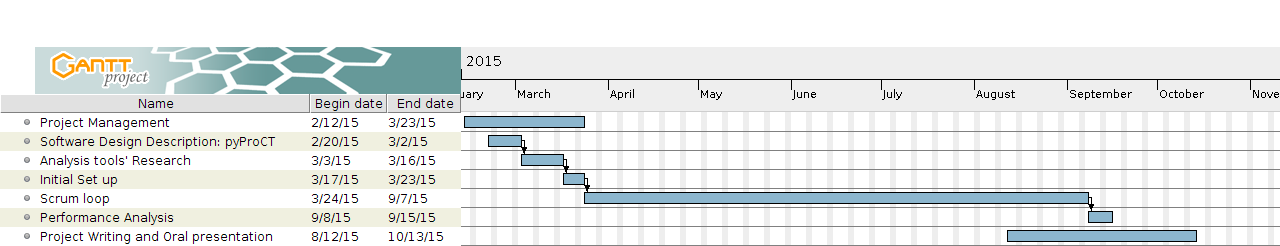
\includegraphics[width=\textwidth]{img/gantt.png}
\caption{Gantt Chart}
\end{figure}
\begin{figure}[h]
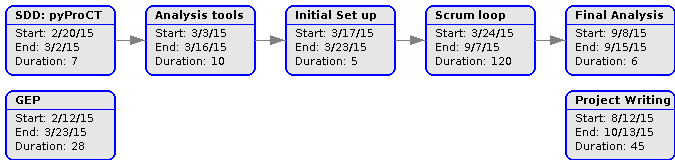
\includegraphics[width=\textwidth]{img/pert.png}
\caption{PERT Chart}
\end{figure}

\FloatBarrier



\chapter{Budget}
\label{sec:budget}
This section describes the required budget for the pyProCT optimization project. It contains a detailed description of the material and human costs. It is divided into: human, hardware and software resources; instead of specifying the costs per tasks, we have decided to use this structure because there are not remarkable differences between the resources used for each task so, grouping them this way, the document will be clearer, will avoid too many subsections and, on the Temporal Planning, the resources needed for each task have already been specified.

\section{Human Resources}


The project was completed by developer and a supervisor. The first worked with an eight-long workday from Monday to Friday. The second's task was to supervise and assess the working process, give advice and help to solve issues. The estimation of the human cost is tied to the work time represented, in this case, by the Gantt Chart and the task description provided on the \hyperref[sec:gantt_pert]{\ref*{sec:gantt_pert} Gantt and PERT charts} section of the temporal planning. 


First is important to note that the Project Management task overlaps with other tasks. However the duration of this section is tied to the programmed schedule of the GEP course, not to the amount of work required to finish it. Thanks to that, we will consider that from 12th February to 12th March the workday is going to be equally distributed amongst the overlapping tasks, which are less work-intensive because they are merely familiarization and research tasks. Similarly, because the results are tied to the development of COMPSs new release, I will start writing the report before having all the results. This way I will have almost everything ready before having the results. 

The defined work period has 176 workdays from 12th February to 13th October (12d + 22d + 22d + 22d + 5d monthly breakdown) amounting to approximately a total of 1400 hours. For the supervisor we estimate 200 hours distributed between meetings, project setup, problem's resolution and correction of this document. 
\\

\begin{center}
	\begin{tabular}{| R{3cm} | L{3cm} | L{3cm} | L{3cm} |}
	\hline
	Role & Price per hour & Time & Cost \\ 
	\hline
	\hline
	Project Developer & 10,00 \euro & 1400h & 14.000,00 \euro \\
	\hline
	Project Supervisor & 30,00 \euro & 100h & 6.000,00 \euro \\
	\hline
	\hline
	Total & - & - & 20.000,00 \euro \\
	\hline
	\end{tabular}
	\captionof{table}{Human Resources Budget} 
\end{center}


\section{Hardware Resources}
\label{sec:hardware_resources}
The hardware resources for this software project are going to be the development device, a laptop, and the testing one, the Mare Nostrum III. It's assumed that the computer used for development has an internet connection and electrical connection. These costs are covered on the total budget together with unexpected costs. However to reduce the budget one possibility would be to consider using the university facilities. The university provides to it's students and developers a free network and plugs which is more than enough in this case.


\makesavenoteenv{tabular}
\begin{center}
	\begin{tabular}{| R{4cm} | L{3cm} | L{2cm} | L{3cm} |}
	\hline
	Product & Price & Useful life & Amortisation \\ 
	\hline \hline
	Mare Nostrum III & 22.700.000,00 \euro & 3 years & 0\protect\footnote{ MareNostrum III is a public infrastructure so users need not to pay to use it} \euro \\
	\hline
	Laptop & 1.200,00 \euro & 3 years & 150,09\footnote{ Given by: Cost / Useful life * Time used on project (664h)} \euro \\
	\hline
	\hline
	Total & 22.701.200,00 \euro & & 150,09 \euro \\
	\hline
	\end{tabular}
	\captionof{table}{Hardware Resources Budget}
\end{center}


\section{Software Resources}
\label{sec:software_resources}

pyProCT is an open source software hosted on a public github repository which can be used without restriction subject to the condition of citing the following article:

%TODO problem with accents in victor name
%Copyright (C) 2012 V�ctor Alejandro Gil Sep�lveda
pyProCT: Automated Cluster Analysis for Structural Bioinformatics
J. Chem. Theory Comput., 2014, 10 (8), pp 3236?3243
DOI: 10.1021/ct500306s \\
As our aim is to improve this software we want to keep it as it is. This means, on one hand, that all the features and optimizations added to it will also be free and public, using no third-party paying software. On the other hand, being it a public software we have decided that the development will allow reproducible research, meaning that all the tools used for analysis are also going to be free and available to anyone trying to reproduce the analysis and optimizations of this project.



\begin{center}
	\begin{tabular}{| R{4cm} | L{3cm} | L{2cm} | L{3cm} |}
	\hline
	Product & Price & Useful life & Amortisation \\ 
	\hline \hline
	Linux Mint 17.1 & 0,00 \euro & - & 0,00 \euro \\
	\hline
	Extrae & 0,00 \euro & - & 0,00 \euro \\
	\hline
	Paraver & 0,00 \euro & - & 0,00 \euro \\
	\hline
	Git & 0,00 \euro& - & 0,00 \euro \\
	\hline
	Github account\footnote{ The repository is public so no premium account is required}& 0,00 \euro & - & 0,00 \euro \\
	\hline
	Texstudio & 0,00 \euro & - & 0,00 \euro \\
	\hline
	GanttProject & 0,00 \euro & - & 0,00 \euro \\
	\hline
	Dia2code (UML drawing)& 0,00 \euro & - & 0,00 \euro \\
	\hline
	Atenea UPC& 0,00 \euro & - & 0,00 \euro \\
	\hline
	Other tools & 0,00 \euro & - & 0,00 \euro \\
	\hline
	\hline
	Total & 0,00 \euro \euro & & 0,00 \euro \euro \\
	\hline
	\end{tabular}
	\captionof{table}{Software Resources Budget}
\end{center}



\section{Total Budget}

Adding up all the cost described on the previous section we get total cost of the project, to which we need to add the VAT, which is 21 \% in Spain. We do not expect big problems or incidents because, as we stated, we aim to use only free software so any modification or change on the task's planning will mainly just add office rental costs (taking into account that the office rental also includes the electricity and internet costs).

To control unexpected events we will add to the Total Cost an amount of money to confront them. These would cover various problems such as: an electricity or internet cost rise, more required office time (rising the rental costs and network/electricity) or, in case of not having enough time, the hiring of supporting help (other developers).


\begin{center}
	\begin{tabular}{| R{7cm} | L{3cm} | L{2cm} | L{3cm} |}
	\hline
	Resource & Price & Useful life & Amortisation \\ 
	\hline \hline
	Hardware & 22.701.200,00 \euro & & 150,09 \euro \\
	\hline
	Software & 0,00 \euro & & 0,00 \euro \\
	\hline
	Developers & 20.000,00 \euro & - & 20.000,00 \euro \\
	\hline
	Office rental & 5.000,00 \euro & - & 5.000,00 \euro \\
	\hline
	Unexpected costs & 3.000,00 \euro & - & 3.000,00\footnote{ Given by: Cost / Useful life * Time used on project (664h)} \euro \\
	\hline
	\hline
	Subtotal & 22.729.200,00 \euro & - & 38.011,70 \euro \\
	\hline
	VAT (21 \%) & 4.773.132,00 \euro & - & 7.982.46 \euro \\
	\hline
	\hline
	Total & 27.502.332,00 \euro & - & 45.994.16 \euro \\
	\hline
	\end{tabular}
	\captionof{table}{Total Budget}
\end{center}

\chapter{Sustainability}
\label{sec:sustainability}
\section{Economic}

An economic assessment has already been described on the Budget Section. The resources used for the development have been kept to a minimum; trying to use all the free software and resources provided by the university, in which a project like this could be developed; being developed by a single person, implying just one salary. The time used, however, could be reduced by having a developer and an analyst. This way on the SCRUB iterations while the developer is working a new feature the analyst could be working on the results of the previous one and so on. A part from that it's difficult to reduce more the amount of work because we have already considered a full-length workday without holidays.

On the major optimization, the COMPSs refactor, we are utilising an already developed framework which eases a lot the amount of work required for it. Thanks to the collaboration with the COMPSs developing team we achieve, as said, a faster implementation, good support, because the framework is currently used, and also we help a good framework as COMPSs to gain more notoriousness and relevance on research projects.

This project will have an 8 in the economical viability area because the cost can hardly be reduced. However, performing a more in-depth ot the risks of the project could help to reduce the budget for unexpected problems.



\section{Social}

On the social dimension we find that the optimization of this software will allow more research teams or enterprises to use it. This is important because on large datasets the amount of time and processing power can be overwhelming for small teams. Even if an optimization as this can not directly change a whole country, it could help universities and developers to waste less time of Supercomputing centers which are quite expensive and so improve their performance and resource disposal and use. As said, these project will not produce better results for the end user but will help the HPC providers.

The optimization covers a necessity as this project is done on BSC demand. So they will benefit from it, harming no one else on the process.

On the social area it will also receive an 8 because it will help to improve and further develop the COMPSs framework on the industry, providing more data, cases of use and information to the BSC/COMPSs development team.

\section{Environmental}

The environmental-related resources of this project are, primarily, two: the Mare Nostrum III supercomputer and the development laptop.

Both resources use electric energy. Theoretically this project will diminish the energy used by the supercomputer, which is quite high, but, in fact, the supercomputer is always running so the impact will be almost negligible, from a power-consumption point of view. However, on smaller scale devices this could in fact reduce a little the amount of energy spent, not worsening it in any case.

The COMPSs framework is used to help the development so we are reusing previously done work, giving the original project more scope and giving it more usage, helping to make the most out of the framework development.

This a software project so no other resources than the electricity used to run it is required. No direct waste is going to be produced by it's use. As it is an open source project aimed to be used or improved the whole project can be reused, both for new projects aiming to reduce even further the power and time consumption and for teams requiring a generic clustering analysis method.

On the resources analysis the project will be awarded with a 9 because the only thing that it's not environmental friendly is the electricity consumed by the Mare Nostrum III and the laptop to run the program and, compared to the average consumption per person nowadays, it's not a big deal.


\chapter{List of References}
\label{sec:docs}


This is a list of the documentation accessed to develop this project. It contains manuals and readmes of the tools, packages and software used.

\begin{itemize}[label={-},labelindent=*,leftmargin=*]
\item \textbf{pyProCT}
\begin{description}[labelindent=10pt,leftmargin=30pt]
\item [Github Readme,] \hfill \\ https://github.com/victor-gil-sepulveda/pyProCT
\item [Dropbox Supporting Information,] \hfill \\ https://dl.dropboxusercontent.com/u/58918851/pyProCT-SupportingInformation.pdf
\end{description}
\item \textbf{pyScheduler}
\begin{description}[labelindent=10pt,leftmargin=30pt]
\item [Github Readme,] \hfill \\
https://github.com/victor-gil-sepulveda/pyScheduler
\item [Python Package Index (pypi),] \hfill \\
https://pypi.python.org/pypi/pyScheduler
\end{description}
\item \textbf{MareNotrum III}
\begin{description}[labelindent=10pt,leftmargin=30pt]
\item [User's guide,] \hfill \\ http://www.bsc.es/support/MareNostrum3-ug.pdf
\end{description}
\item \textbf{COMPSs} \label{subsec:compss_doc}
\begin{description}[labelindent=10pt,leftmargin=30pt]
\item [User Guide,] \hfill \\
http://compss.bsc.es/releases/compss/latest/docs/compss-manual.pdf?tracked=true
\item [Tutorials,] \hfill \\
http://compss.bsc.es/releases/tutorials/?tracked=true
\item [IDE User Guide,] \hfill \\
http://compss.bsc.es/releases/ide/doc/1.2/COMPSs\_IDE\_user\_guide\_v1.2.pdf?tracked=true
\item [Installation,] \hfill \\
http://compss.bsc.es/releases/compss/latest/docs/installation-guide.html?tracked=true
\item [Release Notes,] \hfill \\
http://compss.bsc.es/releases/compss/latest/docs/RELEASE\_NOTES?tracked=true
\end{description}
\item \textbf{Performance Tools}
\begin{description}[labelindent=10pt,leftmargin=30pt]
\item [Extrae User Guide,] \hfill \\ http://www.bsc.es/sites/default/files/public/computer\_science/performance\_tools/extrae-3.1.0-user-guide.pdf
\item [ClusteringSuite intro,] \hfill \\
http://www.bsc.es/ssl/apps/performanceTools/files/docs/T2\_Clustering.pdf
\item [ClusteringSuite manual,] \hfill \\
http://www.bsc.es/sites/default/files/public/computer\_science/performance\_tools/clusteringsuite\_manual.pdf
\item [Paraver introduction,] \hfill \\
http://www.bsc.es/sites/default/files/public/computer\_science/performance\_tools/w1\_introtools.pdf
\item [Paraver internals and details,] \hfill \\
http://www.bsc.es/ssl/apps/performanceTools/files/docs/W2\_Paraver\_details.pdf
\item [Instrumentation,] \hfill \\
http://www.bsc.es/ssl/apps/performanceTools/files/docs/2A\_Instrumentation.pdf
\item [Tools scalability,] \hfill \\
http://www.bsc.es/ssl/apps/performanceTools/files/docs/T1\_Scalability.pdf
\end{description}
\end{itemize}


